\documentclass[withoutpreface]{cumcmthesis}

\begin{document}

\begin{abstractpage}{图论基础与典型问题}

  本文主要研究图论的基础术语和两个典型问题。

  首先,我们陈列了部分图论重要的基础术语,以迅速进入图论研究氛围之中。其次,通过介绍图的矩阵表示,揭示了图在计算机中的输入形式。在这之后,我们分别介绍了最短路径问题及其相关算法( Dijkstra 算法和 Floyd 算法)、最小生成树问题及其相关算法( Kruskal 算法和 Prim 算法),并以具体的示例展示了简单的建模过程。

  \keywords{图 \quad 最短路径 \quad 最小生成树 \quad 邻接矩阵 \quad 关联矩阵}
\end{abstractpage}

\tocpage

\section{图论基本术语}

为了研究图的相关问题,我们需要引入一些特定的规范化的术语。

\subsection{无向图与有向图}

\subsubsection{无向图}

\textbf{无向图}:一个无向图$G$,由非空顶点集$V=\{v_1,v_2,...v_n\}$和边集$E=\{e_1,e_2,...e_m\}$组成,通常记作$G(V,E)$

\textbf{边与顶点}:一条边连接两个顶点(可相同)。故任意一条边可由两个顶点表示:$e_k=(v_i,v_j)$ 。顶点$v_i,v_j$ 称为边$e_k$的端点。边$e_k$与顶点$v_i,v_j$关联。

\textbf{无向图特点}:无向图中的边\textbf{没有方向},即$(v_i,v_j)=(v_j,v_i)$

\textbf{相邻}:有公共端点的边称为相邻的边(\textbf{邻边})。同一条边的两个端点,称为相邻的顶点。

\vspace{-1cm}
\begin{figure}[H]
  \centering
  \subfloat
  {
    \begin{minipage}[t]{0.45\textwidth}
      \centering
      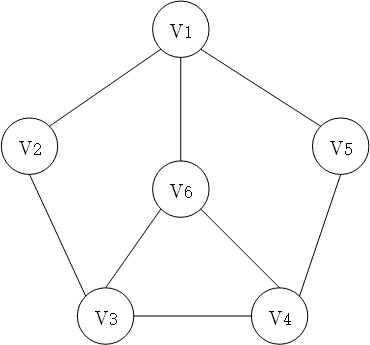
\includegraphics[width=0.9\textwidth]{无向图}
    \end{minipage}
  }
  \subfloat
  {
    \begin{minipage}[t]{0.45\textwidth}
      \centering
      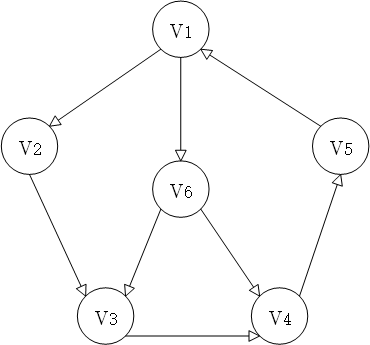
\includegraphics[width=0.9\textwidth]{有向图}
    \end{minipage}
  }
  \caption{无向图(左)与有向图(右)} \label{Fig:1}
\end{figure}

\subsubsection{有向图}

\textbf{弧}:有方向的边称为弧。$a_k=(v_i,v_j)$ 代表弧$a_k$从顶点$v_i$出发指向顶点$v_j$。$v_i$称为$a_k$的始端,$v_j$称为$a_k$的末端。$a_k$称为$v_i$的出弧,称为$v_j$的入弧。

\textbf{有向图}:一个有向图$D$,由非空顶点集$V=\{v_1,v_2,...v_n\}$和弧集$A=\{a_1,a_2,...a_m\}$组成,通常记作$G(V,A)$

\textbf{有向图特点}:有向图中的边\textbf{带有方向},即$(v_i,v_j)\ne(v_j,v_i)$

\textbf{基本图与定向图} :有向图$D=(V,A)$去掉所有边的方向后可以得到对应无向图$G=(V,E)$。称$G$为$D$的基本图,$G$为$D$的定向图。如\cref{Fig:1}所示两图就具有这种关系。

\subsection{简单图,完全图与赋权图}

\textbf{环}:两个端点为同一个顶点的边

\textbf{重边/平行边}:有相同端点的两条或多条边

\textbf{孤立点}:与任何边都不关联的顶点

\textbf{简单图}:无环无重边的图

\begin{figure}[H]
  \centering
  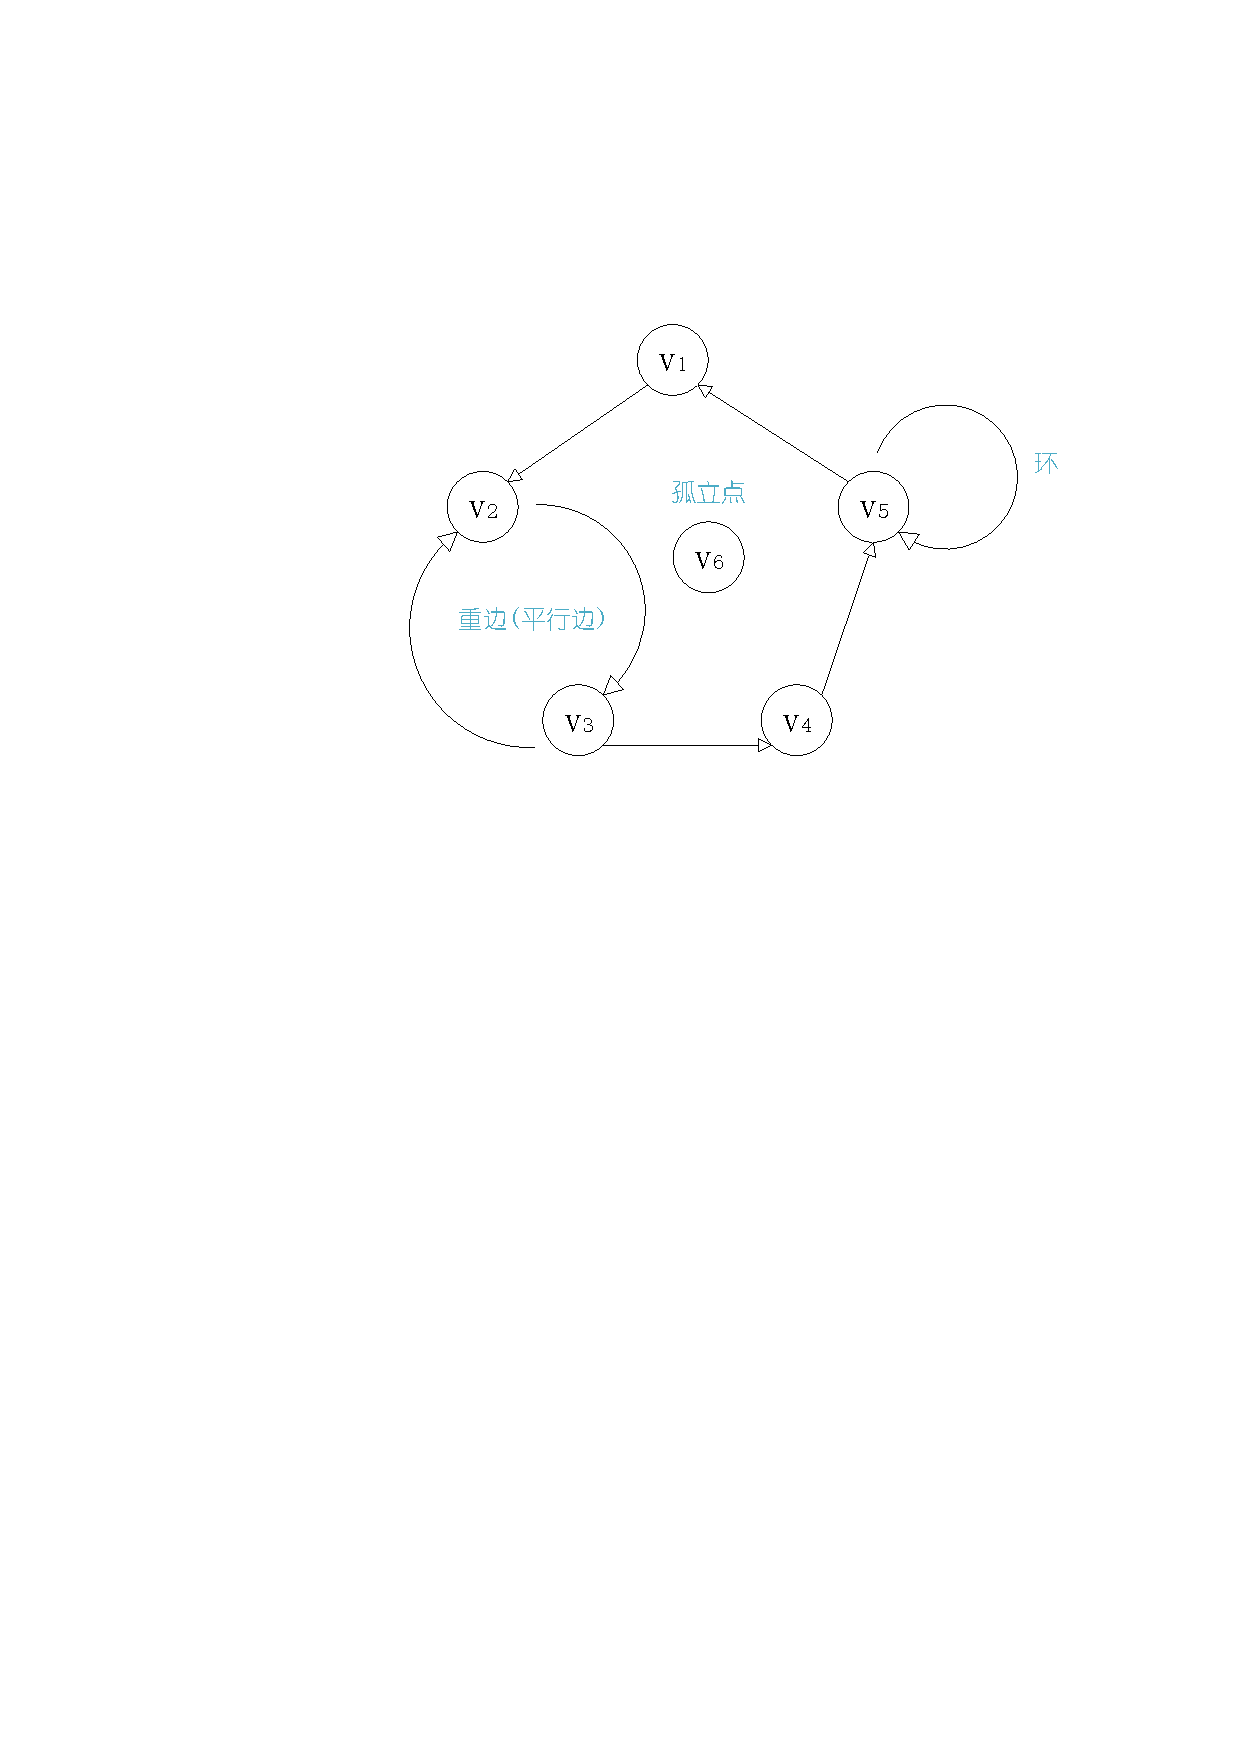
\includegraphics[width=0.6\textwidth]{非简单图}
  \caption{非简单图示例}
\end{figure}

\textbf{完全图}:任意两顶点都相邻的简单图

\textbf{赋权图(网络)}:每条边$e_k$都附加一个权重$w_k$的图 。可记作$N=(V,E,W)$。

\begin{figure}[H]
  \centering
  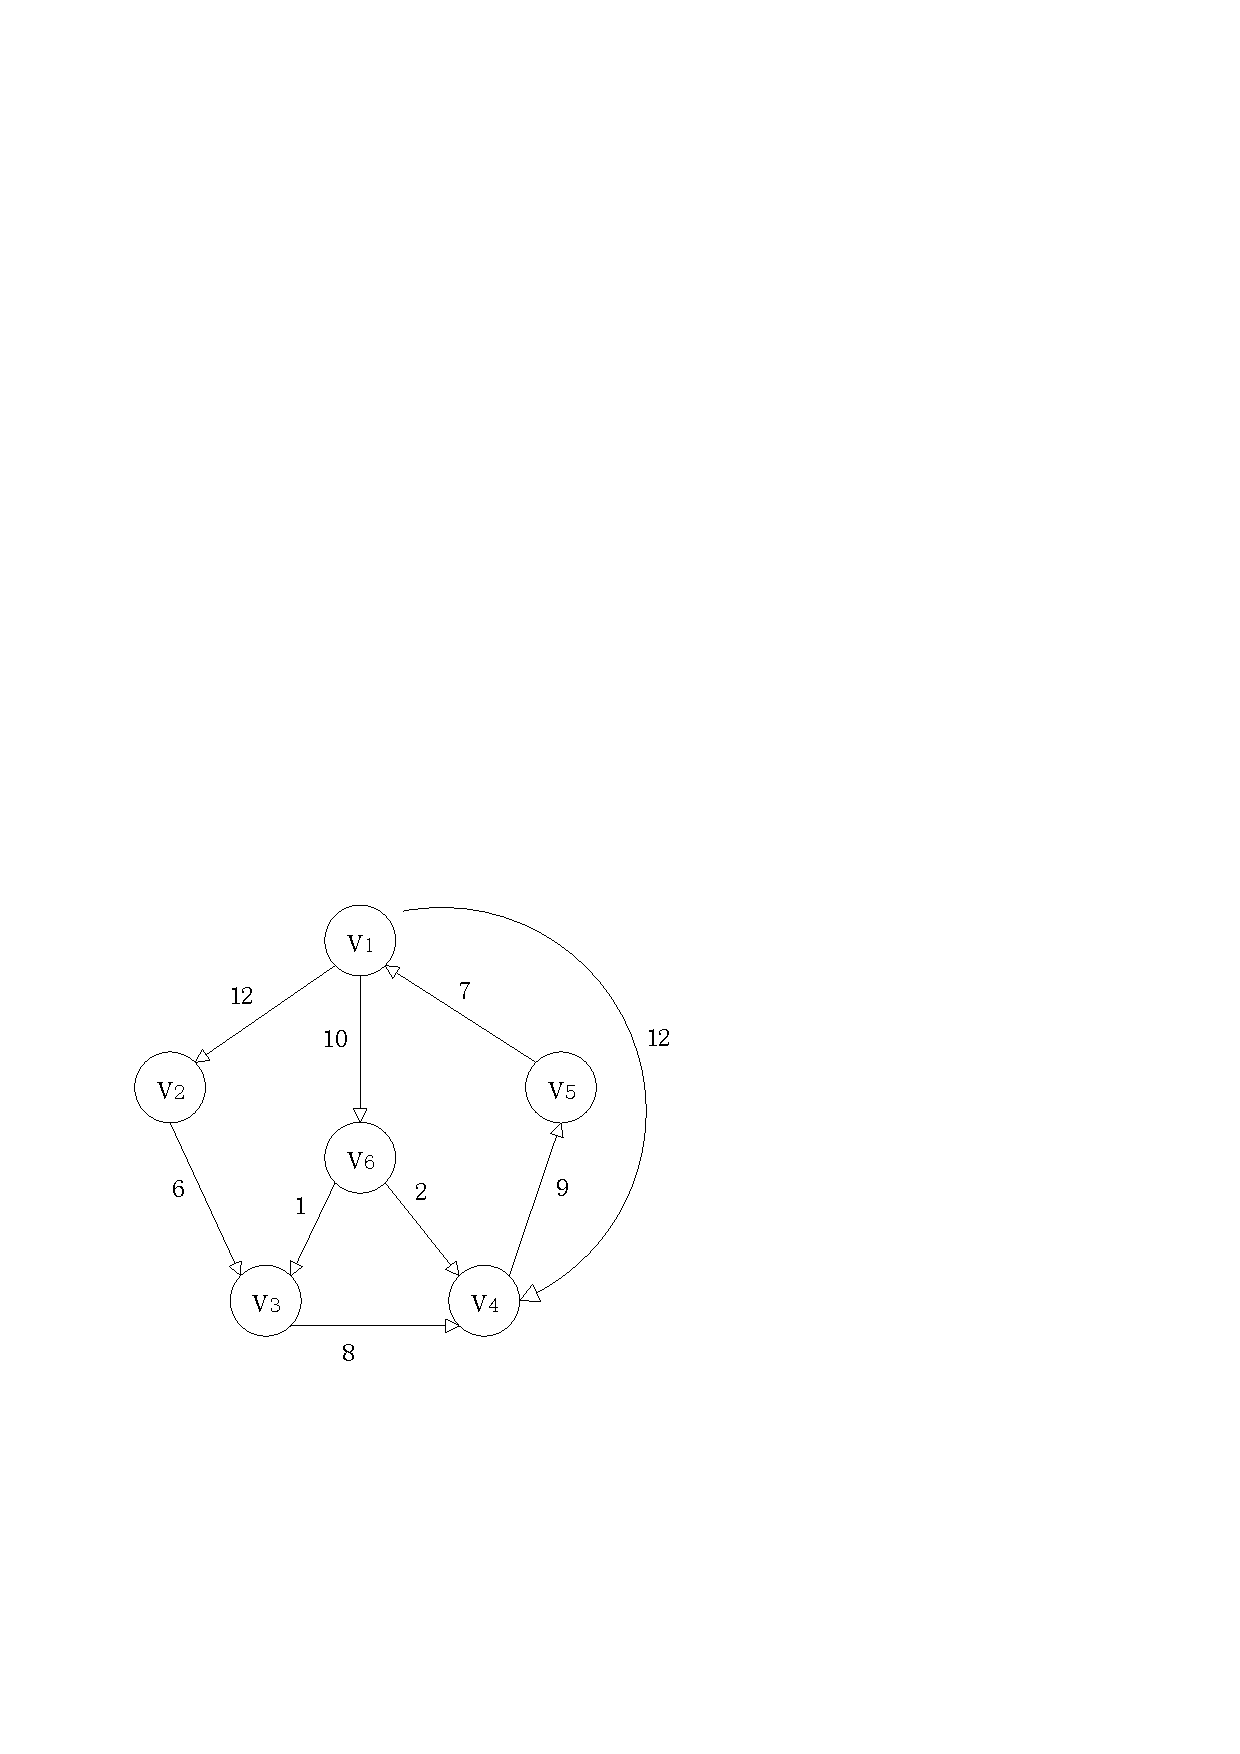
\includegraphics[width=0.5\textwidth]{赋权图}
  \caption{赋权图示例}
\end{figure}

\subsection{顶点的度}

\textbf{顶点$v$的度}:无向图中,与顶点$v$关联的边数;有向图中,弧从顶点$v$出入的总次数。记作$d(v)$

\textbf{出度}:有向图中,从顶点$v$引出的弧的数目。记作$d^+(v)$

\textbf{入度}:有向图中,引入顶点$v$的弧的数目。记作$d^-(v)$

在有向图中,$d(v)=d^+(v)+d^-(v)$

\subsection{子图与图的连通性}

\textbf{子图/母图}:设有图$G_1(V_1,E_1)$,$G_2(V_2,E_2)$.若$G_1$的顶点和边都在$G_2$中能找到,即$V_1\subset V_2,E_1\subset E_2$,则称$G_1$是$G_2$的子图,$G_2$是$G_1$的母图。$G_2$删减若干个顶点和若干条边,可得到$G_1$

\textbf{生成子图/支撑子图}:若$G_1$是$G_2$的子图且两者顶点相同,则称$G_1$是$G_2$的生成子图/支撑子图。$G_2$删减若干条边可生成$G_1$。

\begin{figure}[H]
  \centering
  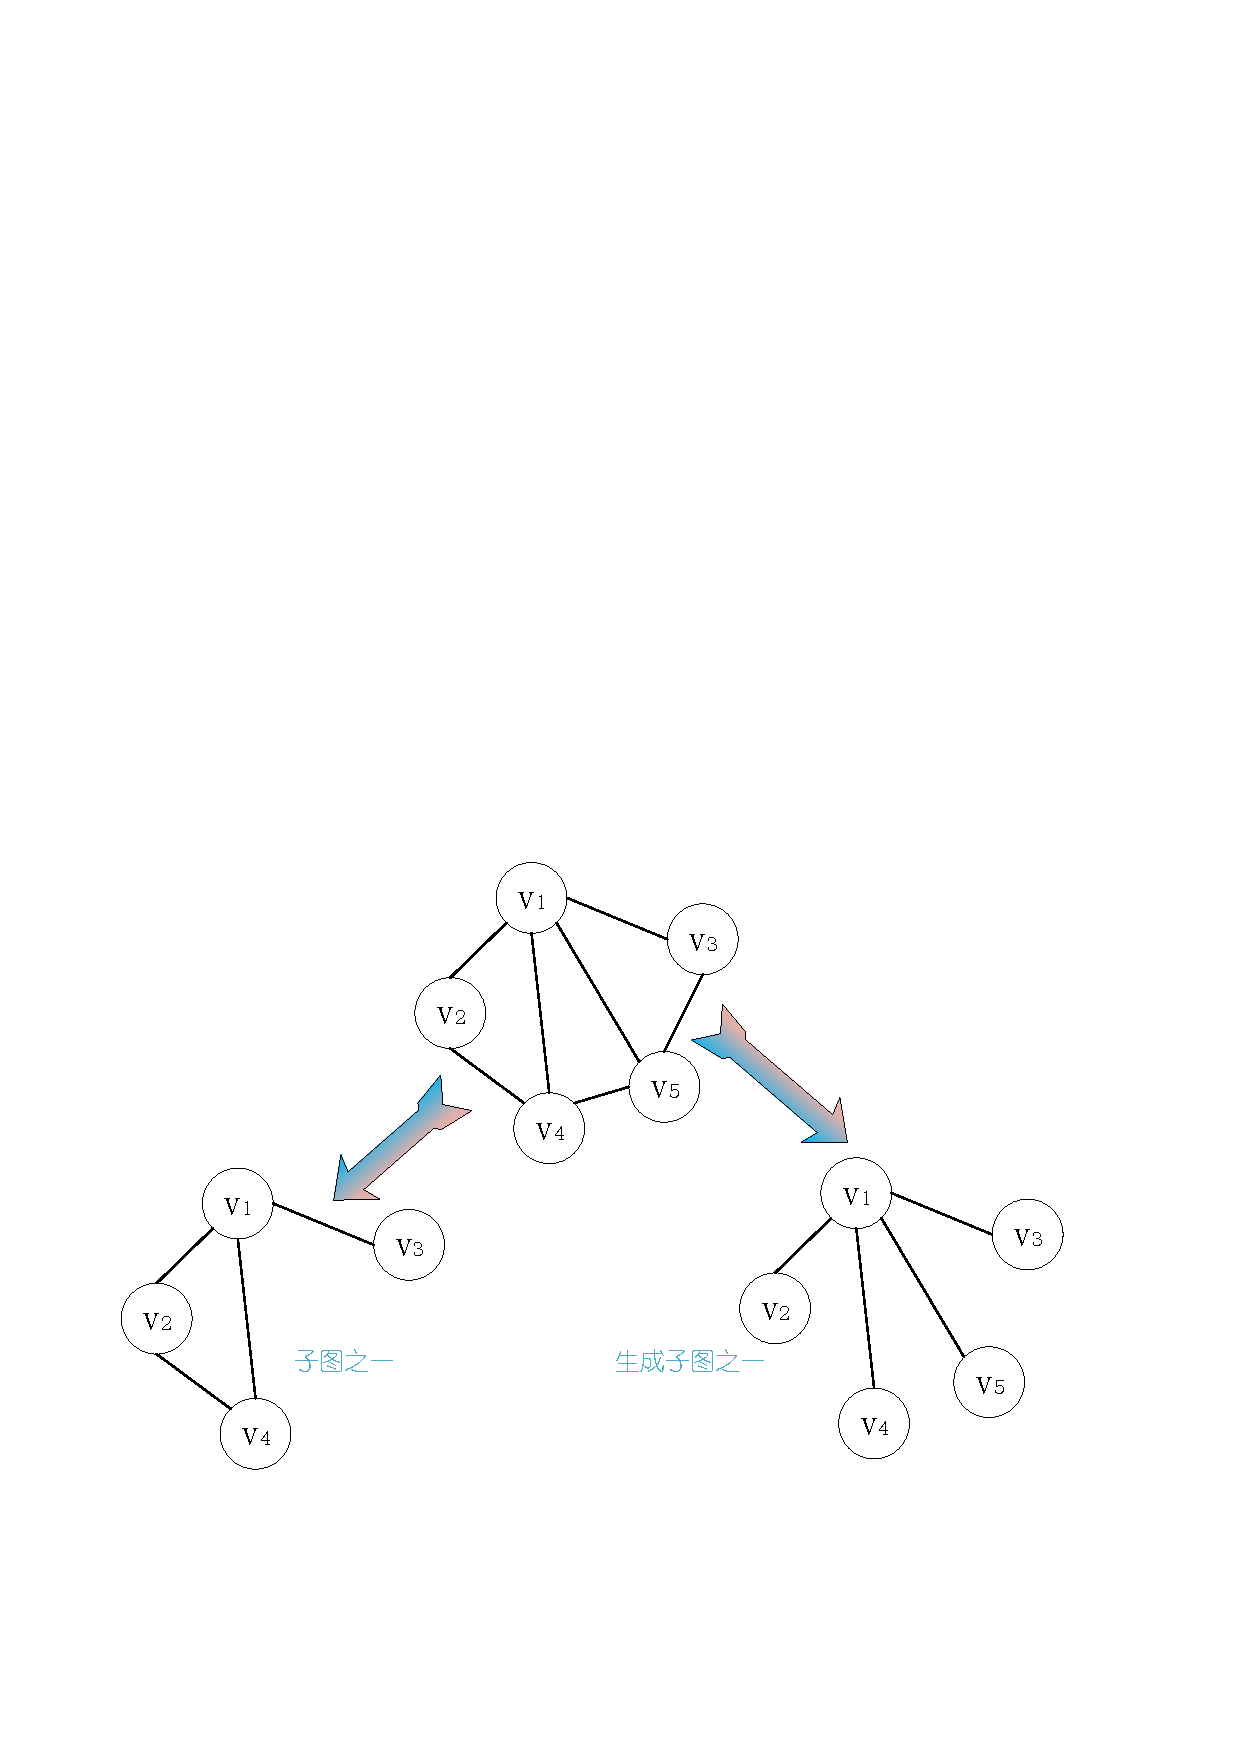
\includegraphics[width=0.8\textwidth]{子图}
  \caption{子图与生成子图示例}
\end{figure}

\textbf{道路/路} :称$v_0e_1v_1e_2...e_kv_k$为从顶点$v_0$到$v_k$的一条道路。其中边$e_i$与顶点$v_{i-1}$,$v_i$相关联。$v_0$为路的起点,$v_k$为路的终点

\textbf{路长}:路所经过的边的条数。即$k$

\textbf{迹}:途径边互异的路。

\textbf{轨道}:途经顶点互异的路。

\textbf{回路}:起点和终点重合的路。

\textbf{圈}:起点和终点重合的轨道。

\textbf{两顶点间的距离}:两顶点间的最短轨道长。

\textbf{连通}:若两顶点间存在路,则称两顶点连通。

\textbf{连通图}:若图的任意两顶点连通,则称该图为连通图。否则称为非连通图。

\textbf{连通分支}:连通图的连通子图

\textbf{强连通图}:若有向图两个顶点$v_i,v_j$间两个方向上都存在路,则称该图为强连通图。

\section{图的矩阵表示}

\subsection{边与顶点的关联矩阵}

设无向图为$G(V,E)$,$V=\{v_1,v_2,...,v_n\}$,$E=\{e_1,e_2,...,e_m\}$,
则其关联矩阵
$$
  M=(m_{ij})_{n\times m}
$$
$$
  m_{ij}=
  \begin{cases} 1 & \mbox{顶点}v_i\mbox{与边}e_j\mbox{关联}  \\
              0 & \mbox{顶点}v_i\mbox{与边}e_j\mbox{不关联}
  \end{cases}
$$

设有向图为$D(V,A)$,$V=\{v_1,v_2,...,v_n\}$,$A=\{a_1,a_2,...,a_m\}$,
则其关联矩阵
$$
  M=(m_{ij})_{n\times m}
$$
$$
  m_{ij}=\begin{cases}
    1  & \mbox{顶点$v_i$为弧$a_j$的始端} \\
    0  & \mbox{顶点$v_i$与弧$a_j$不关联} \\
    -1 & \mbox{顶点$v_i$为弧$a_j$的末端}
  \end{cases}
$$

\subsection{顶点与顶点的邻接矩阵}

设无向非赋权图为$G(V,E)$,$V=\{v_1,v_2,...,v_n\}$

则其邻接矩阵
$$
  W=(w_{ij})_{n\times n}
$$
$$
  w_{ij}=\begin{cases}
    1 & \mbox{顶点$v_i$与$v_j$相邻}      \\
    0 & \mbox{顶点$v_i$与$v_j$不相邻或i=j}
  \end{cases}
$$

设有向非赋权图为$D(V,A)$,$V=\{v_1,v_2,...,v_n\}$

则其邻接矩阵
$$
  W=(w_{ij})_{n\times n}
$$
$$
  w_{ij}=\begin{cases}
    1 & \mbox{弧}(v_i,v_j)\in A               \\
    0 & \mbox{弧}(v_i,v_j)\notin A\mbox{或}i=j
  \end{cases}
$$

设无向赋权图为$G(V,E,W)$,$V=\{v_1,v_2,...,v_n\}$

则其邻接矩阵
$$
  W=(w_{ij})_{n\times n}
$$
$$
  w_{ij}=\begin{cases}
    w_{ij}          & \mbox{顶点$v_i$与$v_j$相邻}      \\
    0\mbox{或}\infty & \mbox{顶点$v_i$与$v_j$不相邻或i=j}
  \end{cases}
$$

有向赋权图的邻接矩阵与无向赋权图类似。

\subsection{总结与举例}

在实际运用中,赋权图顶点与顶点的邻接矩阵的使用更为频繁。

如\cref{Eq:1}中的邻接矩阵$G$对应的无向赋权图
\begin{equation}\label{Eq:1}
  G =
  \begin{bmatrix}
    0  & 0  & 10 & 60   \\
    0  & 0  & 5  & 20 & \\
    10 & 5  & 0  & 1    \\
    60 & 20 & 1  & 0
  \end{bmatrix}
\end{equation}

\begin{figure}[H]
  \centering
  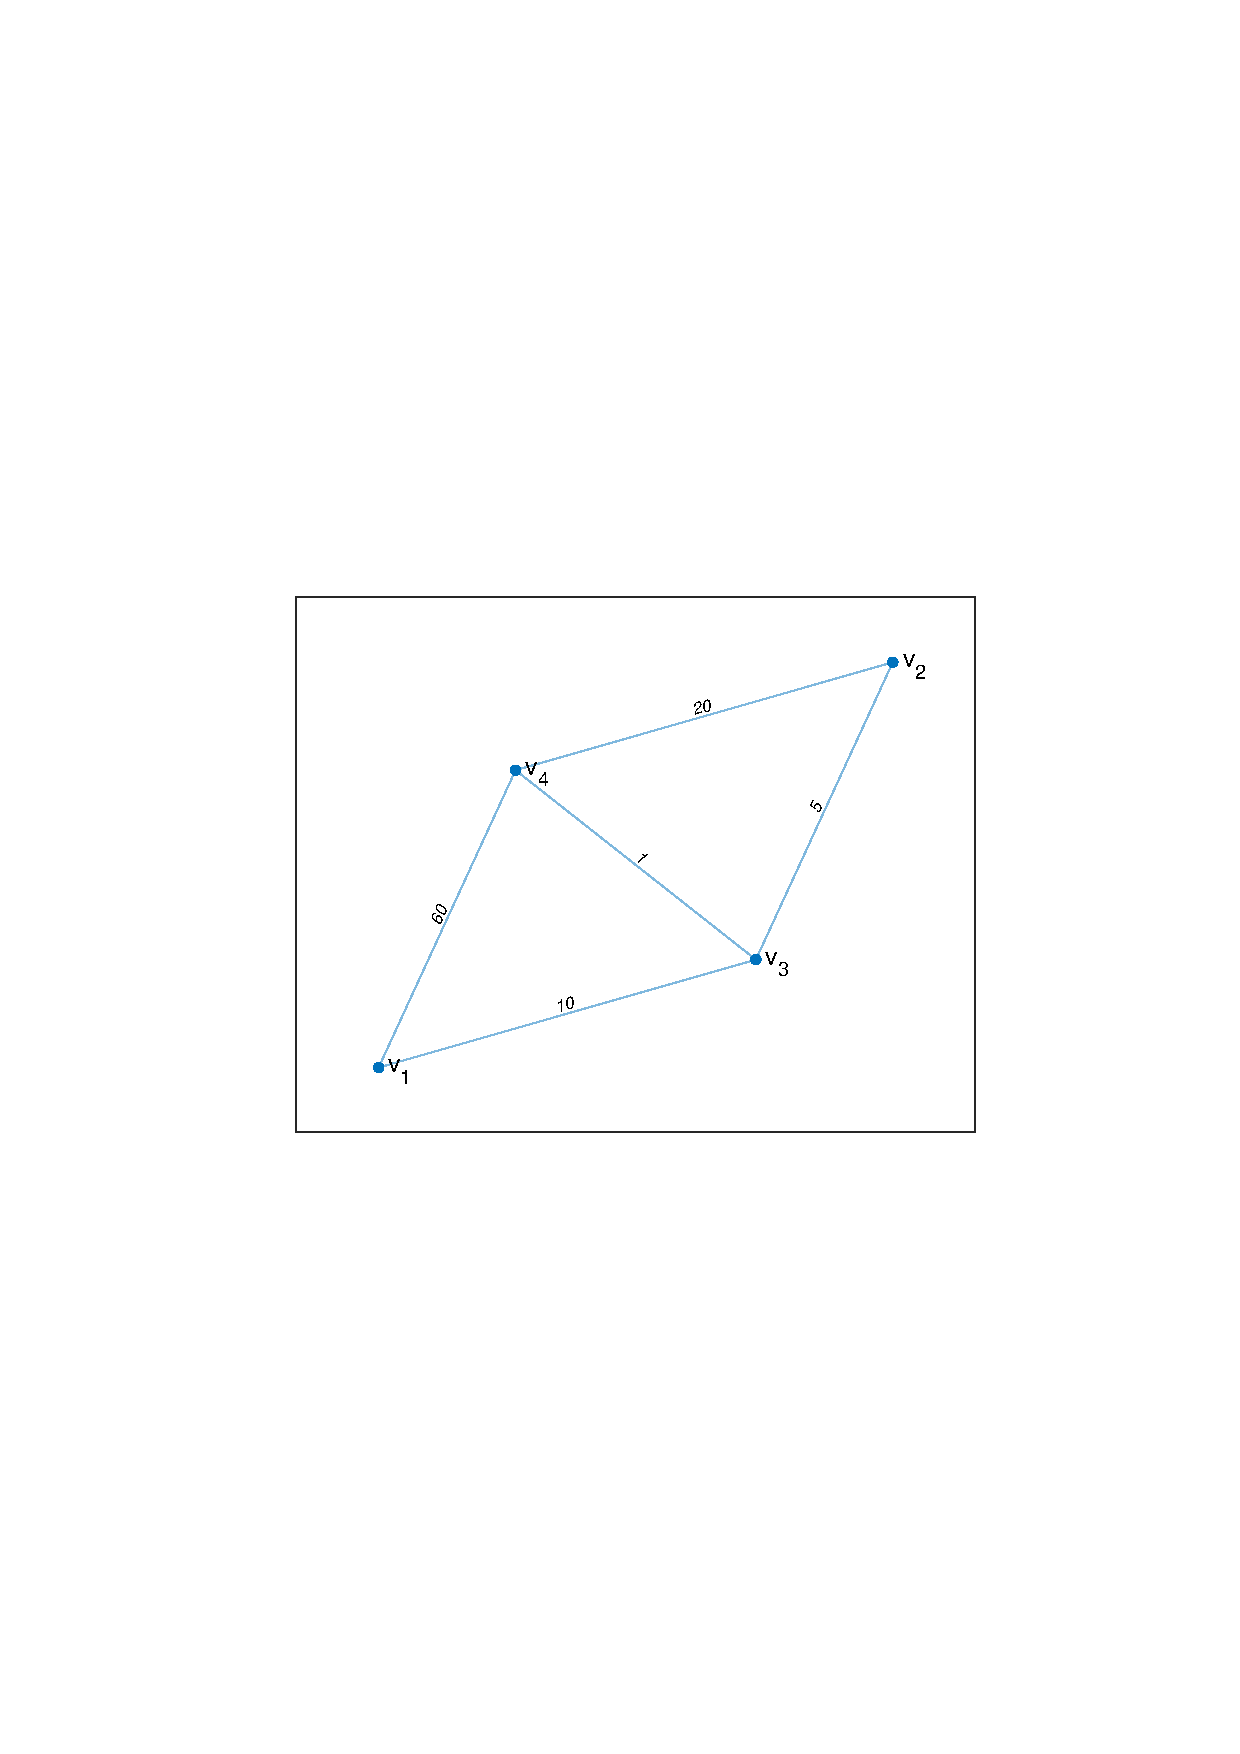
\includegraphics[width=0.5\textwidth]{无向赋权图}
  \caption{邻接矩阵$G$对应的无向赋权图}\label{Fig:5}
\end{figure}

在计算机软件中,通常可以通过邻接矩阵对应的稀松矩阵或者说顶点对创建图。如上面的$G$可以通过$$\mbox{起点向量}\ s = \begin{bmatrix}
    1 \\ 1\\ 2\\ 2\\ 3
  \end{bmatrix} \quad \mbox{终点向量}\ t=\begin{bmatrix}
    3 \\ 4\\ 3\\ 4\\ 4
  \end{bmatrix}
  \quad \mbox{权重向量}\ w = \begin{bmatrix}
    10 \\ 60 \\ 5 \\ 20 \\ 1
  \end{bmatrix}$$
来创建。

\section{最短路径问题}

\subsection{问题简述}

\textbf{路的长度}:赋权图的路经过的边的权重和

\textbf{最短路}:从顶点$v_i$到顶点$v_j$的路径中,长度最小的一条路。

\textbf{顶点间的距离}:顶点$v_i$到顶点$v_j$的最短路的长度。记作$d(u_0,v_0)$

最短路径问题,简而言之就是给定一个赋权图,求某两个顶点之间或所有顶点之间的最短路径。常见的有两种算法可以用于解决最短路径问题: Dijkstra (迪克斯特拉)算法和 Floyd (弗洛伊德)算法。

\vspace{-0.5cm}
\subsection{Dijkstra 算法}

Dijkstra 算法的思想是走一步算一步。最短路径的子路也是最短路径。

\vspace{-0.5cm}
\begin{table}[H]
  \centering
  \caption{算法符号说明}\label{Tab:1}
  \vspace{-0.3cm}
  \begin{tabular}{cc}
    \toprule[1.5pt]
    \makebox[0.3\textwidth][c]{符号说明} & \makebox[0.5\textwidth][c]{意义} \\
    \midrule
    $d_{now}(v)$                     & 从顶点$u_0$当前顶点$v$的路径长度           \\
    $parents(v)$                     & 最短路径中当前顶点$v$的上一个顶点             \\
    $S_i$                            & 含 i 个顶点的最短路径顶点集                \\
    \bottomrule[1.5pt]
  \end{tabular}
\end{table}

\vspace{-0.5cm}
已知赋权无向图$G(V,E,W)$,固定顶点$u_o$,求$u_0$到其余顶点$v$的最短路及距离$d(u_0,v)$。具体的算法步骤如下:

\begin{enumerate}
  \item 令$d_{now}(u_0)=0$.对于其他顶点$v\neq u_0$ ,令$d_{now}(v)=\infty$,$parents(v)=u_0$.令$S_0=\{u_0\}$,$i=0$
  \item 对于所有的$v\notin S_i$,令$\displaystyle d_{now}(v)=\min_{u\in S_i}\{d_{now}(v),d_{now}(u)+w(uv)\}$.若通过$u$更新了$d_{now}(v)$,则令$parents(v)=u$;否则不变。
  \item 寻找$\displaystyle \min_{v\notin S_i} d_{now}(v)$,记该顶点为$u_{i+1}$,令$S_{i+1}=S_i\cup\{u_{i+1}\}$
  \item 若$i=|V|-1$或者$v_0$进入$S_i$,算法终止;否则重复2,3步
\end{enumerate}

\begin{figure}[H]
  \centering
  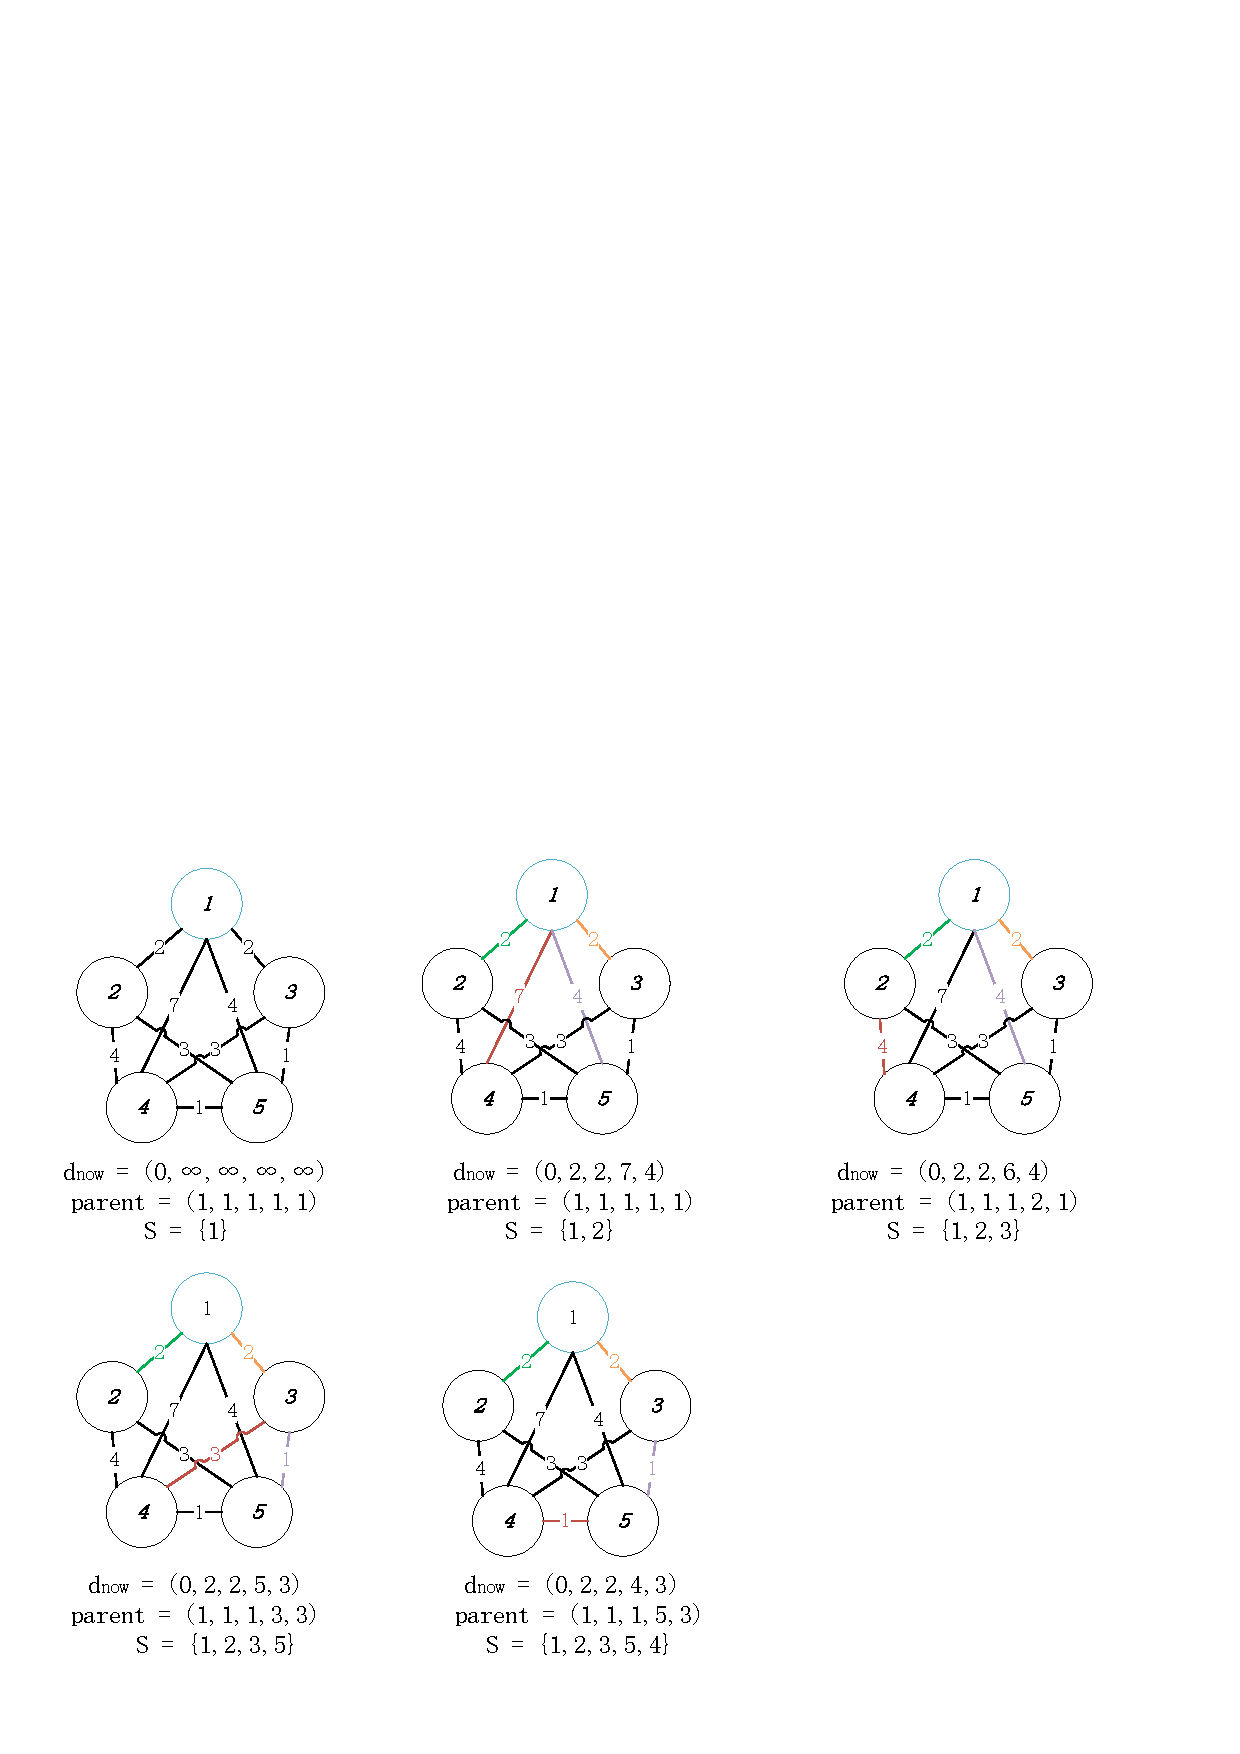
\includegraphics[width=0.72\textwidth]{最短路径1}
  \vspace{-0.2cm}
  \caption{一个 Dijkstra 算法示例}
\end{figure}
\subsection{Floyd 算法}

Floyd 算法的思想是插入中间点。依次将每个顶点作为可能的中间点,插入所有的顶点对之间进行判断,若最短距离更新,则将该点记录下来。直到 n 次之后,得到所有顶点对的最短距离,并通过之间的记录反推最短路径。

\begin{table}[H]
  \centering
  \caption{算法符号说明}\label{Tab:2}
  \vspace{-0.3cm}
  \begin{tabular}{cc}
    \toprule[1.5pt]
    \makebox[0.2\textwidth][c]{符号说明} & \makebox[0.6\textwidth][c]{意义} \\
    \midrule
    $distances$                      & 距离变换矩阵。算法结束后则为顶点之间的最短距离矩阵      \\
    $R$                              & 路由矩阵。记录顶点间的中间点变化               \\
    \bottomrule[1.5pt]
  \end{tabular}
\end{table}

已知赋权无向图$G(V,E,W)$,
求所有顶点对$(u_0,v_0)$之间的最短距离及对应最短路径。具体的算法步骤如下:

\textbf{初始化}:令$distances$为图$G$的带权邻接矩阵.设置不相邻的顶点对对应的$distances$元素为$\infty$.令$R=0_{n\times n}$.$R$对应位置的元素为0,代表两顶点最短路径间无中间点。

\textbf{求距离矩阵和路由矩阵}:从顶点$v_1$开始直到$v_n$,取顶点$v_k$,依次插入到顶点对$(v_i,v_j)$间,若$distances(i,k)+distances(k,j)<distances(i,j)$,说明$v_k$为$(v_i,v_j)$最短路径的中间点。更新$distances(i,j)$为$distances(i,k)+distances(k,j)$.并令$R(i,j)=k$,记录下该中间点。

\textbf{复原路径}:要获得$v_i$与$v_j$的最短路径,只需找到其中间点$v_{R(i,j)}$.再寻找$v_i$与$v_{R(i,j)}$的中间点,$v_j$与$v_{R(i,j)}$的中间点.....重复该过程。

\subsection{示例}

现有A、B、C、D、E五个中转站,它们之间的道路关系及距离如\cref{Tab:3}。请为小明规划从A到E的最短路线。

\begin{table}[H]
  \centering
  \caption{中转站之间的相邻关系及距离}
  \begin{tabular}{|llr|r|llr|}
    \cline{1-3}\cline{5-7}    \rowcolor[rgb]{ .267,  .447,  .769} \textcolor[rgb]{ 1,  1,  1}{\textbf{起点}} & \textcolor[rgb]{ 1,  1,  1}{\textbf{终点}} & \multicolumn{1}{l|}{\textcolor[rgb]{ 1,  1,  1}{\textbf{路程(km)}}} & \cellcolor[rgb]{ 1,  1,  1} & \textcolor[rgb]{ 1,  1,  1}{\textbf{起点}} & \textcolor[rgb]{ 1,  1,  1}{\textbf{终点}} & \multicolumn{1}{l|}{\textcolor[rgb]{ 1,  1,  1}{\textbf{路程(km)}}} \bigstrut \\
    \cline{1-3}\cline{5-7}    A                                                                            & B                                        & 4.5                                                               &                             & B                                        & D                                        & 1.1 \bigstrut                                                               \\
    \cline{1-3}\cline{5-7}    A                                                                            & C                                        & 1.3                                                               &                             & B                                        & E                                        & 0.9 \bigstrut                                                               \\
    \cline{1-3}\cline{5-7}    A                                                                            & D                                        & 3.3                                                               &                             & C                                        & D                                        & 1.9 \bigstrut                                                               \\
    \cline{1-3}\cline{5-7}    A                                                                            & E                                        & 5.6                                                               &                             & C                                        & E                                        & 4.2 \bigstrut                                                               \\
    \cline{1-3}\cline{5-7}    B                                                                            & C                                        & 3.2                                                               &                             & D                                        & E                                        & 2.2 \bigstrut                                                               \\
    \cline{1-3}\cline{5-7}\end{tabular}
  \label{Tab:3}
\end{table}

首先,为了方便处理,我们将A、B、C、D、E五个站点抽象为无向赋权图中的1、2、3、4、5结点,并可得该图的赋权邻接矩阵为
\begin{equation}
  G =
  \begin{bmatrix}
    0   & 4.5 & 1.3 & 3.3 & 5.6 \\
    4.5 & 0   & 3.2 & 1.1 & 0.9 \\
    1.3 & 3.2 & 0   & 1.9 & 4.2 \\
    3.3 & 1.1 & 1.9 & 0   & 2.2 \\
    5.6 & 0.9 & 4.2 & 2.2 & 0
  \end{bmatrix}
\end{equation}

由 Dijkstra 算法或 Floyd 算法可得,由A到E的最短路径为$A\rightarrow C \rightarrow D \rightarrow B \rightarrow E$

最短路径长为5.2 km

\begin{figure}[H]
  \centering
  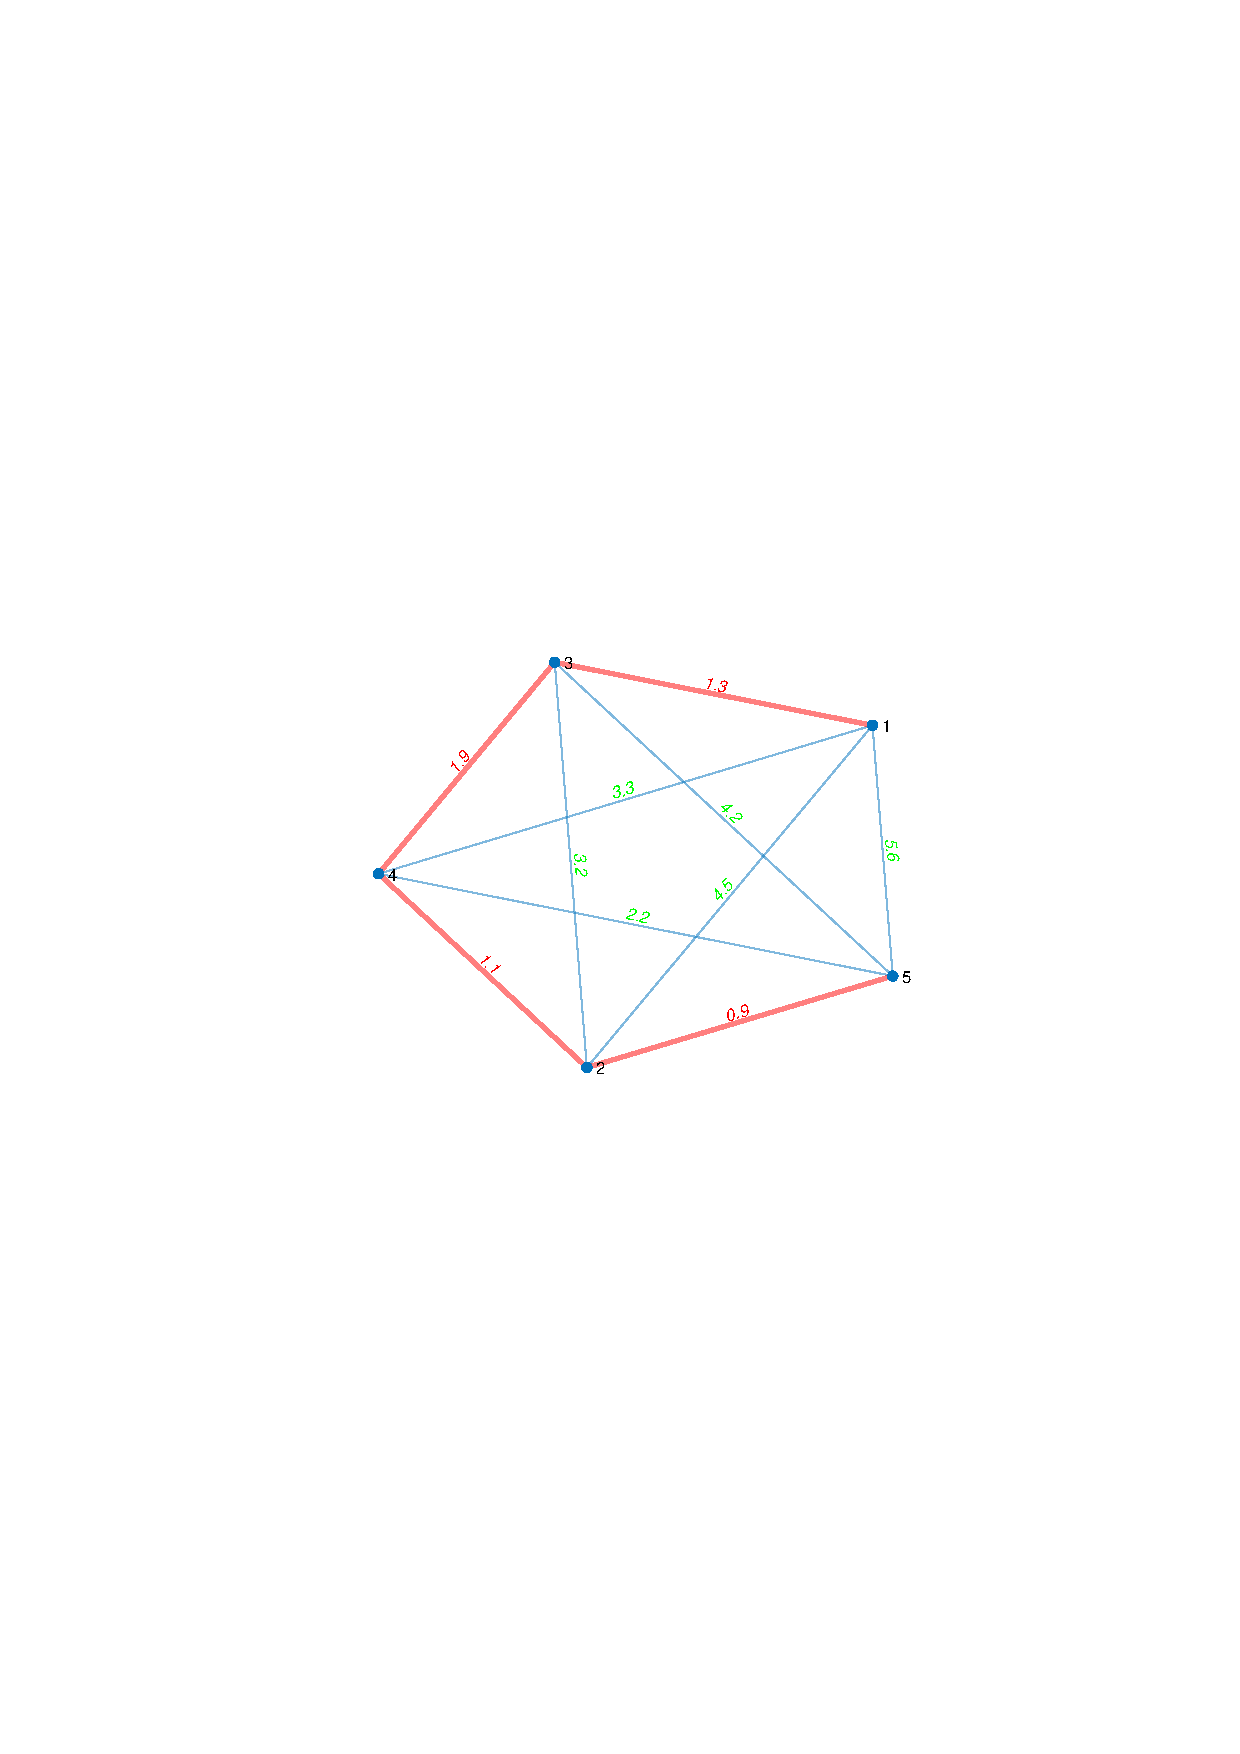
\includegraphics[width=0.6\textwidth]{最短路径2}
  \vspace{-0.2cm}
  \caption{最短路径图示}
\end{figure}


\section{最小生成树问题}

\subsection{问题简述}
\textbf{树}:连通的无圈图

\vspace{0.2cm}
树具有的性质:

\vspace{-0.2cm}
\begin{itemize}
  \item 任意两个不同顶点之间存在唯一的路
  \item 删除任意一条边都不连通
  \item 顶点数=边数+1
  \item 添加任意一条边都会得到唯一的一个圈
\end{itemize}

\textbf{生成树/支撑树}:若图$G$的生成子图$T$是树,则称$T$为$G$的生成树或支撑树。

\vspace{0.2cm}
下面的定理\ref{TH:1}说明,连通图一定存在生成树。


\begin{theorem}\label{TH:1}
  连通图的生成树一定存在。
\end{theorem}

\vspace{-0.6cm}
\begin{proof}
  若连通图$G$无圈,则$G$为本身的生成树。若$G$有圈,任取其一圈,删除其中一条边。易知,$G'$仍旧连通,且圈数-1.重复该步骤,直到得到$G$无圈的连通生成子图,即一个生成树。
\end{proof}

\vspace{-0.4cm}
\textbf{最小生成树}:赋权图$G$的边权和最小的生成树

\vspace{0.1cm}
最小生成树问题,简言之就是找到一棵遍布所有图结点的权重之和最小的树。解决最小生成树问题,常见的算法有 Kruskal (克鲁斯卡尔)算法和 Prim (普里姆)算法。

\subsection{Kruskal 算法}

Kruskal 算法的思想是,每次加一条权值最小的边,并确保不形成圈。

已知赋权无向图$G=(V,E,W)$,其中$V$包含n个顶点。求$G$的最小生成树。具体的算法步骤如下:

\begin{enumerate}
  \item 选取$e_1\in E$,使得$e_1$为权值最小的边
  \item 若$e_1,e_2,···,e_i$已经选好,则从$E-\{e_1,e_2,···,e_i\}$中选取$e_{i+1}$,使得$\{e_1,e_2,···,e_i,e_{i+1}\}$中无圈,且$e_{i+1}$是$E-\{e_1,e_2,···,e_i\}$中权值最小的边
  \item 直至选得$e_{n-1}$为止
\end{enumerate}

\subsection{Prim 算法}

Prim 算法基于这样一个现实:最小生成树中包含$G$的所有顶点。

\begin{table}[H]
  \centering
  \caption{算法符号说明}\label{Tab:4}
  \vspace{-0.3cm}
  \begin{tabular}{cc}
    \toprule[1.5pt]
    \makebox[0.3\textwidth][c]{符号说明} & \makebox[0.5\textwidth][c]{意义} \\
    \midrule
    $V_{added}$                      & 已加入最小生成树的顶点                    \\
    $E_{added}$                      & 已加入最小生成树的边                     \\
    \bottomrule[1.5pt]
  \end{tabular}
\end{table}


已知赋权无向图$G=(V,E,W)$,其中$V$包含n个顶点。求$G$的最小生成树。具体的算法步骤如下:

$$ V_{added}=\{v_1\} $$
$$E_{added}= \varnothing $$

$while\ V_{added}\neq V:$

\qquad 寻找最小权值边$pv$,其中,$p\in V_{added},v\in V-V_{added}$
$$V_{added}=V_{added}+\{v\}$$
$$E_{added}=E_{added}+\{pv\}$$

\subsection{示例}

有9个村庄,将其编号为1-9,它们之间的道路长如\cref{Tab:5}所示,请问应该如何架设通信线,才能通信线线长最小。
\begin{table}[htbp]
  \centering
  \caption{村庄之间的道路长}
    \begin{tabular}{|ccc|r|ccc|}
\cline{1-3}\cline{5-7}    \rowcolor[rgb]{ .267,  .447,  .769} \textcolor[rgb]{ 1,  1,  1}{\textbf{村庄}} & \textcolor[rgb]{ 1,  1,  1}{\textbf{村庄}} & \textcolor[rgb]{ 1,  1,  1}{\textbf{距离(km)}} & \cellcolor[rgb]{ 1,  1,  1} & \textcolor[rgb]{ 1,  1,  1}{\textbf{村庄}} & \textcolor[rgb]{ 1,  1,  1}{\textbf{村庄}} & \textcolor[rgb]{ 1,  1,  1}{\textbf{距离(km)}} \bigstrut\\
\cline{1-3}\cline{5-7}    \rowcolor[rgb]{ .851,  .882,  .949} 1     & 2     & 2     & \cellcolor[rgb]{ 1,  1,  1} & 2     & 3     & 4 \bigstrut\\
\cline{1-3}\cline{5-7}    1     & 3     & 1     &       & 2     & 9     & 1 \bigstrut\\
\cline{1-3}\cline{5-7}    \rowcolor[rgb]{ .851,  .882,  .949} 1     & 4     & 3     & \multicolumn{1}{l|}{\cellcolor[rgb]{ 1,  1,  1} } & 3     & 4     & 1 \bigstrut\\
\cline{1-3}\cline{5-7}    1     & 5     & 4     &       & 4     & 5     & 1 \bigstrut\\
\cline{1-3}\cline{5-7}    \rowcolor[rgb]{ .851,  .882,  .949} 1     & 6     & 4     & \cellcolor[rgb]{ 1,  1,  1} & 5     & 6     & 5 \bigstrut\\
\cline{1-3}\cline{5-7}    1     & 7     & 2     &       & 6     & 7     & 2 \bigstrut\\
\cline{1-3}\cline{5-7}    \rowcolor[rgb]{ .851,  .882,  .949} 1     & 8     & 5     & \cellcolor[rgb]{ 1,  1,  1} & 7     & 8     & 3 \bigstrut\\
\cline{1-3}\cline{5-7}    1     & 9     & 4     &       & 8     & 9     & 5 \bigstrut\\
\cline{1-3}\cline{5-7}    \end{tabular}%
  \label{Tab:5}
\end{table}

通过\cref{Tab:5}中的数据建立图模型,利用 Kruskal 算法或 Prim 算法求得最小生成树如\cref{Fig:8}所示,即应该铺设线路的道路为 (1,2), (1,3), (1,7), (2,9), (3,4), (4,5), (6,7), (7,8)。最小线长为13 km. 

\begin{figure}[H]
  \centering
  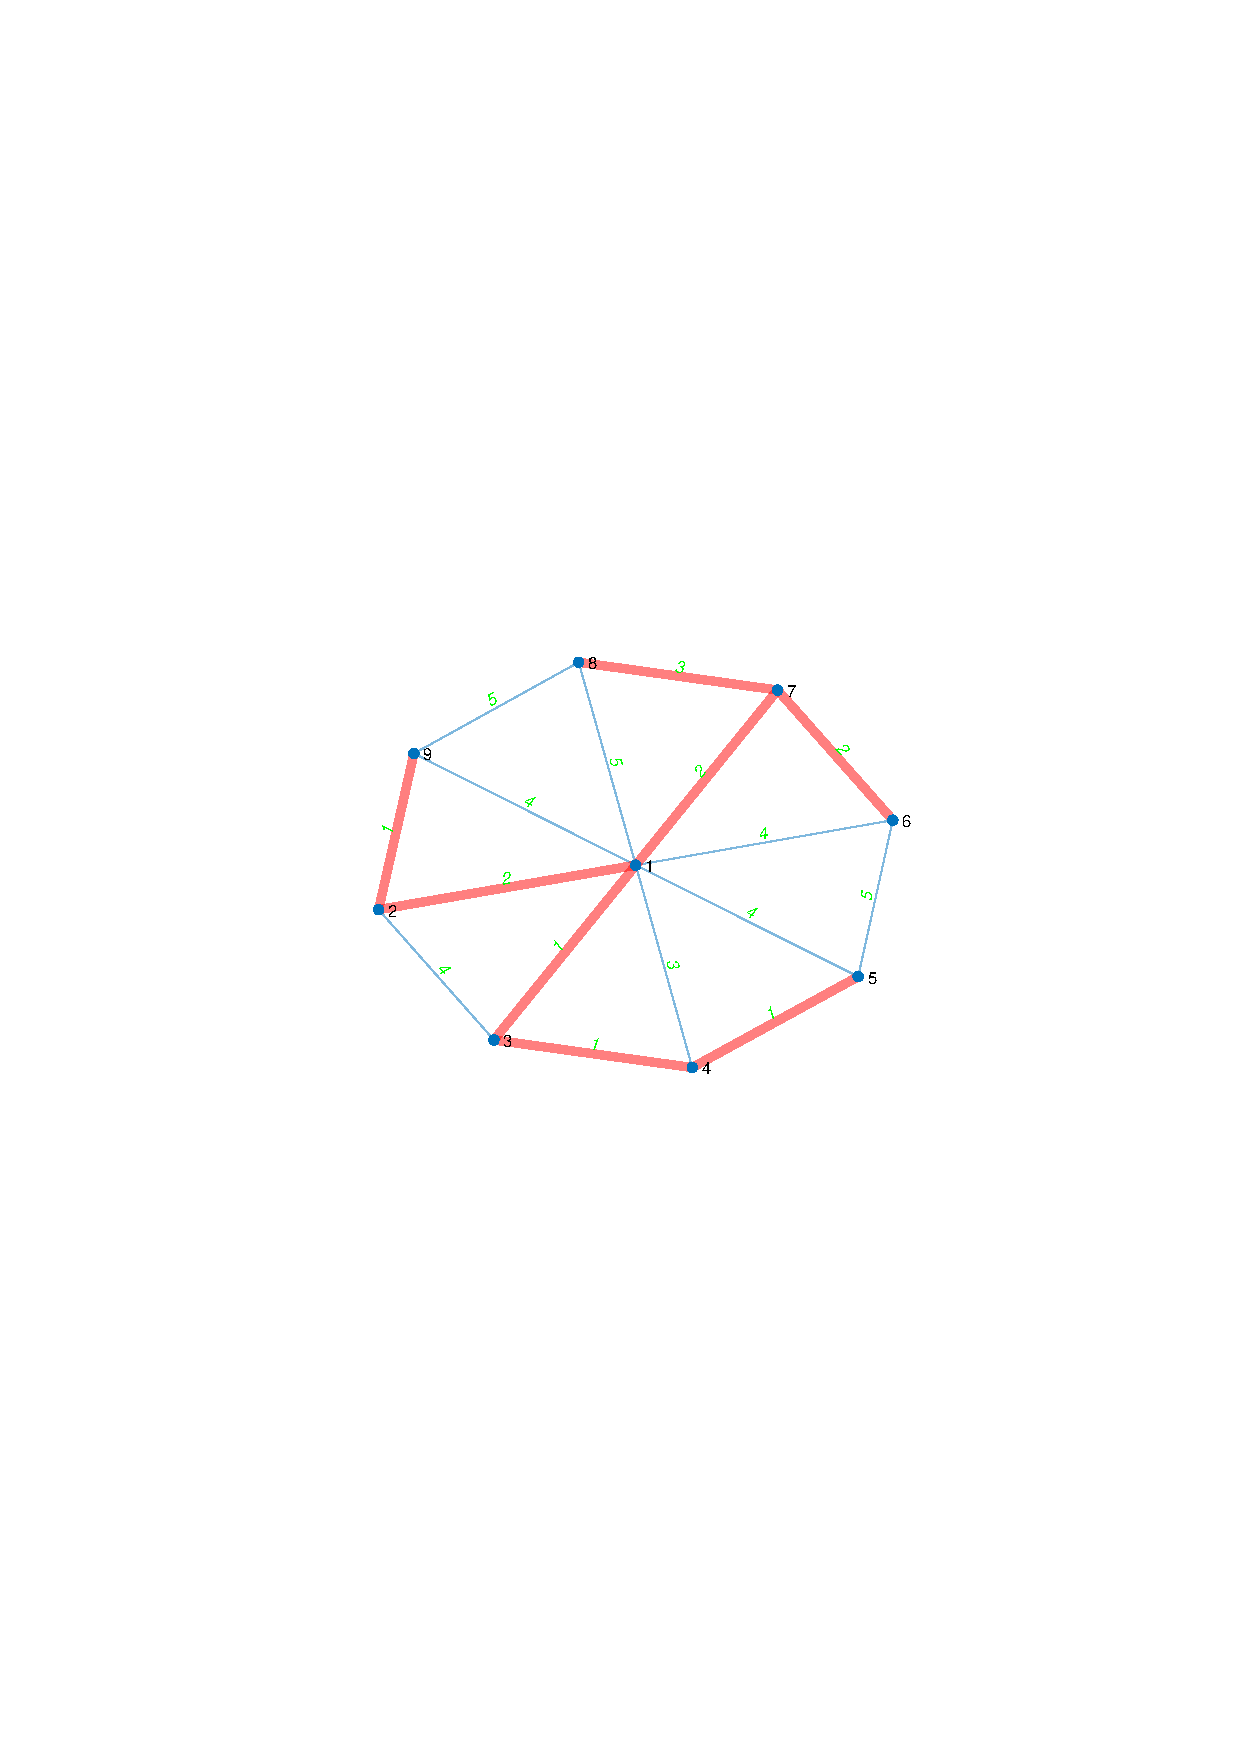
\includegraphics[width=0.5\textwidth]{最小生成树}
  \vspace{-0.2cm}
  \caption{最小生成树图示}\label{Fig:8}
\end{figure}

\appendix
\section{Matlab代码}
  \begin{lstlisting}[language=matlab ,caption={Dijkstra算法} ]
  function [path, distance] = Dijkstra(G, u0, v0)
  % Dijkstra算法求最短路径
  
    % 初始化参数
    n = G.numnodes;
    nodes = 1:n;
    i = 0;
    d_now = ones(n, 1) * inf;
    d_now(u0) = 0;
    parents = ones(n, 1) * u0;
    in_s = u0;

    history = [];
    % 遍历所有终点或v0进入最短路径集
    while (i ~= n - 1) && ~(ismember(v0, in_s))
        not_in_s = setdiff(nodes, in_s);
        for v = not_in_s
            for u = in_s
                % 查找uv间的边
                uv_index = G.findedge(u, v);
                if uv_index
                    % 边存在则获取权
                    w = min(G.Edges.Weight(uv_index));
                    % 计算新的最短距离
                    d_now(v) = min([d_now(v), d_now(u) + w]);
                    if d_now(u) + w <= d_now(v)
                        % 距离发生改变
                        parents(v) = u;
                        % 记录变化
                        history = [history; [u, v]];
                    end
                end
            end
        end
        % 寻找最短距离的顶点
        tmp = d_now;
        tmp(in_s) = inf;
        [~, new_u] = min(tmp);
        new_u = new_u(1);
        % 添加最短路径顶点
        in_s = union(new_u, in_s);
        i = i + 1;
    end

    % 倒溯最短路径
    last = v0;
    path = v0;

    while last ~= u0
        k = find(history(:, 2) == last);
        last = history(k(end), 1);
        path = [last, path];
    end

    distance = d_now(v0);
  end
  \end{lstlisting}

  \begin{lstlisting}[language=matlab ,caption={Floyd算法} ]
  function [distances, paths] = Floyd(G)
  % Floyd算法求所有顶点对之间的最短路径

    % 矩阵初始化
    distances = G.adjacency('weighted');
    n = length(distances);
    distances(distances == 0) = inf;
    distances(1:n + 1:end) = 0;
    R = zeros(n);

    for k = 1:n
        for i = 1:n
            for j = 1:n
                % 插点更新
                if distances(i, k) + distances(k, j) < distances(i, j)
                    distances(i, j) = distances(i, k) + distances(k, j);
                    R(i, j) = k;
                end
            end
        end
    end

    distances = full(distances);

    % 复原路径
    paths = returnPaths(R);

    for i = 1:n
        for j = 1:n
            if i ~= j
                % 添加起点和终点
                paths{i, j} = [i paths{i, j} j];
            else
                paths{i, j} = i;
            end
        end
    end
end

  function paths = returnPaths(R)
      % 根据路由矩阵返回最短路径矩阵
      n = length(R);
      paths = cell(n);

      for i = 1:n
          for j = 1:n
              paths{i, j} = parse(i, j);
          end
      end
      
    % 递归推导最短路径
    function path = parse(i, j)
        p = R(i, j);
        if p == 0
            path = [];
        else
            left = parse(i, p);
            right = parse(p, j);
            path = [left, p, right];
        end
    end

  end
  \end{lstlisting}

  \begin{lstlisting}[language=matlab ,caption={Kruskal算法} ]
  function [resultgraph, minw] = Kruskal(G)
  % Kruskal算法求最小生成树
  
      % 初始化参数
      W = full(G.adjacency("weighted"));
      n = length(W);
      W(W == 0) = inf;
      minw = 0;
      resultgraph = graph();
      i = 1;
  
      while i < n
          % 寻找最小权值边
          w_min = min(W, [], "all");
          [index_x, index_y] = find(W == w_min, 1);
          % 添加最小权值边
          resultgraph = resultgraph.addedge(index_x, index_y, w_min);
          % 判断添加该边后图是否有圈
          if hascycles(resultgraph)
              % 有圈则删除该边,并标记pass
              resultgraph = resultgraph.rmedge(index_x, index_y);
              W(index_x, index_y) = inf;
              W(index_y, index_x) = inf;
          else
              % 无圈则保持,并标记pass
              W(index_x, index_y) = inf;
              W(index_y, index_x) = inf;
              minw = minw + w_min;
              i = i + 1;
          end
      end
  end
  \end{lstlisting}

  \begin{lstlisting}[language=matlab ,caption={} ]
  function [resultgraph, minw] = Prim(G)
  % Prim算法求解最小生成树
  
      % 初始化参数
      W = full(G.adjacency("weighted"));
      n = length(W);
      W(W == 0) = inf;
      V = 1:n;
      V_added = [1];
      E_added = [];
      minw = 0;
  
      % 直至V和V_added相等
      while ~isequal(V, sort(V_added))
          tmp = W;
          V_not_added = setdiff(V, V_added);
          % 圈定p,v范围
          tmp(V_not_added, :) = inf;
          tmp(:, V_added) = inf;
          w_min = min(tmp, [], "all");
          minw = minw + w_min;
          [p, v] = find(tmp == w_min, 1);
          % pv边标记pass
          W(p, v) = inf;
          W(v, p) = inf;
          % 更新
          V_added = union(V_added, v);
          E_added = [E_added; p, v, w_min];
      end
  
      s = E_added(:, 1);
      t = E_added(:, 2);
      w = E_added(:, 3);
      resultgraph = graph(s, t, w);
  end
  \end{lstlisting}

  \begin{lstlisting}[language=matlab ,caption={示例代码} ]
  clc,clear

  %% 无向赋权图通过邻接矩阵创建
  figure(1);
  % 输入邻接矩阵A
  A = [ 0 0 10 60;
      0 0 5 20;
      10 5 0 1;
      60 20 1 0];	
      
  % 输入结点名
  nodes=["v_1","v_2","v_3","v_4"];
  
  % 使用邻接矩阵A和结点名nodes创建赋权无向图
  G = graph(A,nodes);
  
  % plot函数显示图
  plot(G,"EdgeLabel",G.Edges.Weight,"NodeFontSize",12);
  
  %% 无向赋权图通过顶点对创建
  figure(2);
  % 输入一个顶点
  s = [1 1 2 2 3];
  
  % 输入另一个顶点
  t = [3 4 3 4 4];
  
  % 输入结点名
  nodes = ["v_1","v_2","v_3","v_4"];
  
  % 输入权值
  weights = [10 60 5 20 1];
  
  % 使用顶点对s,t和结点名nodes创建赋权无向图
  G = graph(s,t,weights,nodes);
  
  % plot函数显示图
  plot(G,"EdgeLabel",G.Edges.Weight,"NodeFontSize",12)
  
  %% 最短路径
  % 输入图的顶点对
  s = [1,1,1,1,2,2,2,3,3,4];
  t = [2,3,4,5,3,4,5,4,5,5];
  w = [4.5,1.3,3.3,5.6,3.2,1.1,0.9,1.9,4.2,2.2];
  
  figure(3);
  % 创建并绘制图
  G=graph(s,t,w);
  fig1=plot(G,"EdgeLabel",G.Edges.Weight,'EdgeLabelColor','green');
  
  % 使用Dijkstra算法求得最短路径并在图中标出
  [path,distance]=Dijkstra(G,1,5);
  highlight(fig1,path,'EdgeColor','red','LineWidth',2,"EdgeLabelColor","red");
  
  % 使用Floyd算法求所有最短路径
  [distances,paths]=Floyd(G);
  
  %% 最小生成树
  s1 = [1,1,1,1,1,1,1,1,2,2,3,4,5,6,7,8];
  t1 = [2,3,4,5,6,7,8,9,3,9,4,5,6,7,8,9];
  w1 = [2,1,3,4,4,2,5,4,4,1,1,1,5,2,3,5];
  G = graph(s1,t1,w1);
  
  % Kruskal算法求解最小生成树
  [min_tree, min_w] = Kruskal(G);
  
  figure(4);
  % 绘图并加粗最小生成树
  fig2 = plot(G, "EdgeLabel", G.Edges.Weight, 'EdgeLabelColor', 'green');
  highlight(fig2, min_tree, "EdgeColor", "red", "LineWidth", 4);
  
  figure(5);
  % Prim算法求解最小生成树
  [tree_min,w_min] = Prim(G);
  
  % 绘图并加粗最小生成树
  fig3=plot(G,"EdgeLabel",G.Edges.Weight,'EdgeLabelColor','green');
  highlight(fig3,tree_min,"EdgeColor","red","LineWidth",4);
  \end{lstlisting}

  \section{Python 代码}

  \begin{lstlisting}[language=python ,caption={导库} ]
  import networkx as nx
  import numpy as np
  import pandas as pd
  \end{lstlisting}

  \begin{lstlisting}[language=python ,caption={通过顶点对创建无向赋权图} ]
  # 输入边和权
  s1 = [f"$v_{i}$" for i in [1, 1, 2, 2, 3]]
  t1 = [f"$v_{i}$" for i in [3, 4, 3, 4, 4]]
  w1 = [10, 60, 5, 20, 1]
  edges = list(zip(s1, t1, w1))
  
  # 创建空图并添加顶点和边权
  G1 = nx.Graph()
  G1.add_weighted_edges_from(edges)
  
  # 计算顶点位置
  pos1 = nx.spring_layout(G1)

  # 绘制无权图
  nx.draw(G1, pos1, with_labels=True, font_size=14)
  
  # 追加绘制权
  labels = nx.get_edge_attributes(G1, 'weight')
  fig1 = nx.draw_networkx_edge_labels(G1, pos1, edge_labels=labels, font_color="red")
  \end{lstlisting}

  \begin{lstlisting}[language=python ,caption={Dijkstra算法} ]
  def Dijkstra(G, u0, v0):
  """利用Dijkstra计算最短路径和距离"""

    # 初始化参数
    n = G.number_of_nodes()
    nodes = list(range(1, n + 1))
    d_now = np.ones(n) * np.inf
    d_now[u0 - 1] = 0
    parents = [u0 for i in range(n)]
    s = set()
    s.add(u0)
    history = []
    i = 0

    # 遍历所有终点或v0进入最短路径顶点集
    while (i != n - 1) or (v0 not in s):
        not_s = set(nodes) - s
        for v in not_s:
            for u in s:
                try:
                    # 检查顶点u,v间是否有边
                    w = G.edges[u, v]['weight']
                except:
                    pass
                else:
                    d_now[v - 1] = min([d_now[v - 1], d_now[u - 1] + w])
                    if d_now[u - 1] + w <= d_now[v - 1]:
                        # 顶点最短值改变,记录改变
                        parents[v - 1] = u
                        history.append([u, v])

        # 寻找当前的最小距离点,并加入s集合
        tmp = d_now.copy()
        in_s_index = [i - 1 for i in s]
        tmp[in_s_index] = np.inf
        new_u = np.argmin(tmp) + 1
        s.add(new_u)
        i = i + 1

    # 拼接最终的最短路径
    last = v0
    path = [v0]
    history = np.array(history)
    while last != u0:
        k = np.where(history[:, 1] == last)
        last = history[k[-1][-1], 0]
        path.append(last)

    path = path[-1::-1]
    distance = d_now[v0 - 1]
    return path, distance


  # 输入边和权
  edges = [(1, 2, 4.5), (1, 3, 1.3), (1, 4, 3.3), (1, 5, 5.6), (2, 3, 3.2), (2, 4, 1.1), (2, 5, 0.9), (3, 4, 1.9),
            (3, 5, 4.2), (4, 5, 2.2)]
  
  # 创建空图并添加顶点和边权
  G2 = nx.Graph()
  G2.add_weighted_edges_from(edges)
  
  # 计算顶点位置
  pos2 = nx.spring_layout(G2)

  # 绘制无权图
  nx.draw(G2, pos2, with_labels=True, font_size=14)

  # 绘制最短路径
  path, distance = Dijkstra(G2, 1, 5)
  shortest_edges = []
  for i in range(np.size(path) - 1):
      shortest_edges.append((path[i], path[i + 1]))
  nx.draw_networkx_edges(G2, pos2, edgelist=shortest_edges, edge_color='red')

  # 追加绘制权
  labels = nx.get_edge_attributes(G2, 'weight')
  fig2 = nx.draw_networkx_edge_labels(G2, pos2, edge_labels=labels, font_color="green")
  \end{lstlisting}

  \begin{lstlisting}[language=python ,caption= ]
  def returnPaths(R):
  """根据路由矩阵还原路径"""

    def parse(i, j):
        """递归解析i,j顶点最短路径"""
        p = R[i, j]
        if p == 0:
            path = []
        else:
            path = [p]
            left = parse(i, p - 1)
            right = parse(p - 1, j)
            path.extend(right)
            for num in left[-1::-1]:
                path.insert(0, num)
        return path

    n, n = np.shape(R)
    paths = [[] for i in range(n)]
    for i in range(n):
        for j in range(n):
            paths[i].append(parse(i, j))
    return paths

  def Floyd(G):
  """Floyd算法求所有顶点间的最短路径"""

    # 初始化矩阵
    distances = nx.to_numpy_matrix(G)
    n, n = np.shape(distances)
    distances[distances == 0] = np.inf
    row, col = np.diag_indices_from(distances)
    distances[row, col] = 0
    R = np.zeros((n, n), dtype=int)

    # 插点更新
    for k in range(n):
        for i in range(n):
            for j in range(n):
                if distances[i, k] + distances[k, j] < distances[i, j]:
                    distances[i, j] = distances[i, k] + distances[k, j]
                    R[i, j] = k + 1

    # 复原路径
    paths = returnPaths(R)

    # 路径添加起点和终点
    for i in range(n):
        for j in range(n):
            if i != j:
                paths[i][j].append(j + 1)
                paths[i][j].insert(0, i + 1)
            else:
                paths[i][j] = [i + 1]
    return distances, paths


  distances, paths = Floyd(G2)
  # 最短路径长
  n = G2.number_of_nodes()
  d_df = pd.DataFrame(distances, index=range(1, n + 1), columns=range(1, n + 1))
  d_df
  # 最短路径集
  p_df = pd.DataFrame(paths, index=range(1, n + 1), columns=range(1, n + 1))
  p_df
  \end{lstlisting}

  \begin{lstlisting}[language=python ,caption={Kruskal算法} ]
  def Kruskal(G):
  """Kruskal算法求解最小生成树"""
    # 初始化参数
    W = nx.to_numpy_matrix(G)
    n, n = np.shape(W)
    W[W == 0] = np.inf
    minw = 0
    resultgraph = nx.Graph()
    i = 1

    while i < n:
        # 寻找最小权值边
        w_min = np.min(W)
        index_x, index_y = [
            np.where(W == w_min)[0][0],
            np.where(W == w_min)[1][0]
        ]
        # 添加最小权值边
        resultgraph.add_edge(index_x + 1,
                             index_y + 1,
                             weight=G.edges[index_x + 1,
                                            index_y + 1]['weight'])
        try:
            # 判断添加该边后图是否有圈
            nx.find_cycle(resultgraph)
        except:
            # 无圈则保持,并标记pass
            W[index_x, index_y] = np.inf
            W[index_y, index_x] = np.inf
            minw = minw + w_min
            i = i + 1
        else:
            # 有圈则删除该边,并标记pass
            resultgraph.remove_edge(index_x + 1, index_y + 1)
            W[index_x, index_y] = np.inf
            W[index_y, index_x] = np.inf

    return resultgraph, minw


  # 输入边和权
  edges = [(1, 2, 2), (1, 3, 1), (1, 4, 3), (1, 5, 4), (1, 6, 4), (1, 7, 2), (1, 8, 5), (1, 9, 4),(2, 3, 4), (2, 9, 1), (3, 4, 1), (4, 5, 1), (5, 6, 5), (6, 7, 2), (7, 8, 3), (8, 9, 5)]

  # 创建空图并添加顶点和边权
  G3 = nx.Graph()
  G3.add_weighted_edges_from(edges)

  # 计算顶点位置
  pos3 = nx.spring_layout(G3)

  # 绘制无权图
  nx.draw(G3, pos3, with_labels=True, font_size=14)
  
  # Kruskal算法求解最小生成树
  min_tree, wmin = Kruskal(G3)
  
  # 绘制最小生成树
  nx.draw_networkx_edges(G3, pos3, edgelist=min_tree.edges, edge_color="red", width=3)
  
  # 追加绘制权
  labels = nx.get_edge_attributes(G3, 'weight')
  edges = nx.draw_networkx_edge_labels(G3,
                                       pos3,
                                       edge_labels=labels,
                                       font_color="green")
  \end{lstlisting}

  \begin{lstlisting}[language=python ,caption={Prim算法} ]
  def Prim(G):
  """Prim算法求解最小生成树"""
    # 初始化参数
    W = nx.to_numpy_matrix(G)
    n, n = np.shape(W)
    W[W == 0] = np.inf
    V = set(range(1, n + 1))
    V_added = {1}
    E_added = []
    minw = 0

    # 直至V和V_added相等
    while V != V_added:
        tmp = W.copy()
        V_not_added = V - V_added
        # 圈定p,v范围
        index_x = [i - 1 for i in V_not_added]
        tmp[index_x, :] = np.inf
        index_y = [i - 1 for i in V_added]
        tmp[:, index_y] = np.inf
        w_min = np.min(tmp)
        minw = minw + w_min
        p, v = np.where(tmp == w_min)[0][0] + 1, np.where(
            tmp == w_min)[1][0] + 1
        # pv边标记pass
        W[p - 1, v - 1] = np.inf
        W[v - 1, p - 1] = np.inf
        # 更新
        V_added.add(v)
        E_added.append((p, v, w_min))

    resultgraph = nx.Graph()
    resultgraph.add_weighted_edges_from(E_added)
    return resultgraph, minw


  # 绘制无权图
  nx.draw(G3, pos3, with_labels=True, font_size=14)
  
  # Prim算法求解最小生成树
  min_tree, minw = Prim(G3)
  
  # 绘制最小生成树
  nx.draw_networkx_edges(G3, pos3, edgelist=min_tree.edges, edge_color="red", width=3)
  
  # 追加绘制权
  labels = nx.get_edge_attributes(G3, 'weight')
  p_edges = nx.draw_networkx_edge_labels(G3,
                                          pos3,
                                          edge_labels=labels,
                                          font_color="green")
  \end{lstlisting}
\end{document}